\section{System's Perspective}

\subsection{Design and Architecture of MiniTwit}
The MiniTwit system is designed in a way that allows us to separate the models, the views and the controllers,
as seen in figure \ref{fig:minitwit}. This is done to reduce the coupling between our components and to make 
it simpler to extend the functionality of the application.  

\begin{figure}[H]
    \centering
    \captionsetup{justification=centering,margin=1cm}
    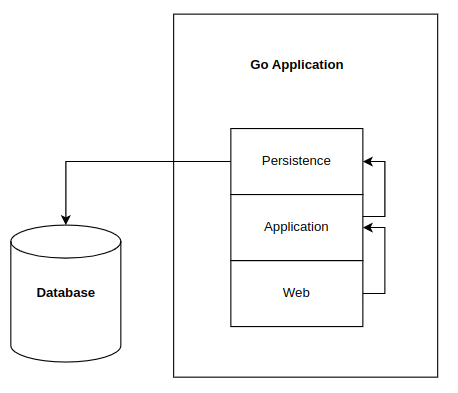
\includegraphics[width=0.8\linewidth]{report/images/system_architecture.png}
    \caption{MiniTwit Architecture}
    \label{fig:minitwit}
\end{figure}

The application is implemented using the RESTful API, which means that when a user interacts with a part of the 
view, an HTTP request is sent. This request is then handled by the corresponding controller, and it ensures 
that the correct action is taken. This could be a call to a function that updates the model, and the return of 
an appropriate HTTP response. 


\subsection{Dependencies of MiniTwit system}
% deployment diagram??

%%% NOTE:
The application is hosted at Digital Ocean. We use Docker Swarms to scale the application horizontally. For 
monitoring the application we use Grafana. Logging is done using Elastic Search and Kibana. Additionally, we have a Redis database 
that stores sessions and the integer 'latest' and a postgreSQL database storing other information, such as 
the registered users and created messages. 

\subsection{Important Interactions of Subsystems}

\subsection{Current state of the system}

\subsection{Project License}